\section{Theoretical Analysis}
\label{sec:analysis}

\par First of all, we need to analyse the circuit in general. It has thirteen meshes, of which four are elementar, nine nodes and eleven branches (seven resistors, one independent voltage source, $V_A$, one independent current source, $I_D$, one voltage controlled current source $I_B$ and one current controlled voltage source $V_C$. In order to discover the currents and the voltages in nodes we could use Kirchhoff's Current Law (KCL) and the Kirchhoff's Voltage Law (KVL), but we used two methods (that are based on these two laws), which are explained in the following sections.

\subsection{Mesh method}
\label{mesh method}

To use this method we need to identify the loops, as we can see in the image above. Each one of the loops have one associated current, that we call $I_A$, $I_B$, $I_C$ and $I_D$. To discover the value of this currents we need to analyse each mesh by itself, but we have to beware that components that make part of more than one loop have a current that is influenced by the currents of those loops. For example for the first loop, we have to sum the voltage of each component. In the voltage source we know that the voltage is $V_A$, for the resistor, $R_1$, we use the Ohm's Law and we get that $V_1 = R_1$. However for the others two resistor, we will use the Ohm's Law again and we will notice that they make part of two loops. The voltage that goes through the resistor is multiplication the value of the resistor and the current. Looking at the branches in between two nodes we can see that both of the loop currents go through the branch but in opposite directions. The current with the same direction as the branch current (+ $\rightarrow$ -) will have a positive sign and the loop current going through the opposite direction will have a negative sign. We do the same for the resistor $R_4$. For the others two loops we did the same way and we got 3 equations in total:
 
\begin{center}
    \begin{equation}
       I_1(R_1+ R_4 + R_3)-I_2 R_3-I_3 R_4=-V_A 
      \end{equation}
\end{center}
\begin{center}
    \begin{equation}
          I_1(-R_3 K_b)+I_2(K_b R_3-1)=0 
    \end{equation}
\end{center}

\begin{center}
    \begin{equation}
        I_1(-R_4)+I_3(-K_c-R_6-R_7+R_4)=0 
    \end{equation}
\end{center}


%esquema mesh method
\begin{figure}[h] \centering
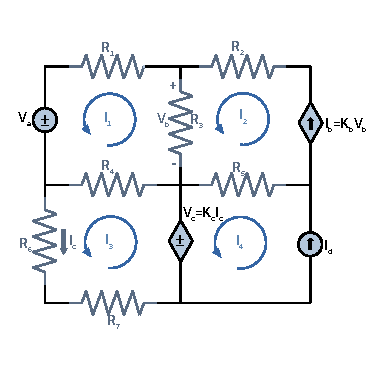
\includegraphics[width=0.8\linewidth]{mesh.pdf}
\caption{Mesh method}
\label{fig:forced}
\end{figure}



To solve this system of linear equations we used Octave and we get the following values:

%tabela malhas Is
\begin{table}
  \centering
  \begin{tabular}{|l|r|}
    \hline    
    {\bf Name} & {\bf Value [A or V]} \\ \hline
    I1 & 0.00022339172\\ \hline 
I2 & 0.00023403434\\ \hline 
I3 & -0.00099456437\\ \hline 

  \end{tabular}
  \label{tab:op}
\end{table}

The last calculations are presented in the table below 

%tabela malhas - calculos
\begin{table}[h]
  \centering
  \begin{tabular}{|l|r|}
    \hline    
    {\bf Name} & {\bf Value [A or V]} \\ \hline
    Vc & -7.9685230178\\ \hline 
I2 & 0.03289187116\\ \hline 

  \end{tabular}
  \label{tab:op}
\end{table}

\subsection{Node Voltage Method}
\label{node method}

\par A really powerful way of analyzing circuits is called the Node Voltage Method, which is based on Kirchhoff's Current Law (KCL).

%imagem metodo nos
\begin{figure}[h] \centering
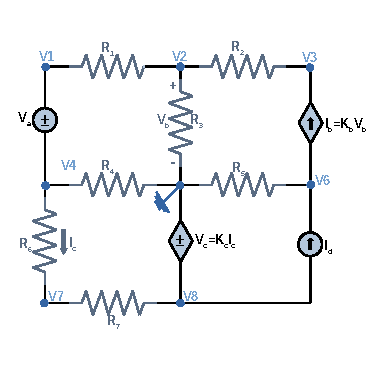
\includegraphics[width=0.8\linewidth]{nodes.pdf}
\caption{Node method: labeling of the nodes}
\label{fig:forced}
\end{figure}

To begin with, we should start by explaining what node voltage means. When we use the term node voltage, we are referring to the potential difference between two nodes of a circuit. This is still a voltage, it's not anything too strange. We start by labelling the nodes with numbers and assigning each with its own variable, $V_1$, $V_2$, etc. Then, we select one of the nodes in the circuit to be the reference node and call this reference node the ground node. It gets a ground symbol in the schematic. The potential of the ground node is defined to be $0 V$. The choice of the reference node is somewhat arbitrary, but it's always best to choose it based on its connections to voltage sources, because by this selection we already know the node voltages of other nodes, i.e. the ones that the reference node is connected to them by voltage sources. We chose for the ground node node 5, since it is connected to dependent voltage source $V_c$ and three different resistors. Therefore, $V_5 = 0 V$. Choosing node 5 as the ground node also allows us to state that $V_2 = V_b$, for instance. After that is done, we apply KCL for each node. Taking all of this into account, we end up with the following equations

\begin{center}
    \begin{equation}  
      V_1 - V_4 = V_a
       \end{equation}
\end{center}

\begin{center}
  \begin{equation}
    V_1(-G_1) + V_2(G_1+G_2+G_3) + V_3(-G_2) = 0
  \end{equation}
\end{center}

\begin{center}
  \begin{equation}
    V_2(-K_b-G_2) + V_3(G_2)= 0
  \end{equation}
\end{center}

\begin{center}
  \begin{equation}
    V_2(K_b) + V_6(G_5) = I_d
  \end{equation}
\end{center}

\begin{center}
  \begin{equation}
    V_4(G_6) + V_7(-G_6-G_7) + V_8(G_7) = 0
  \end{equation}
\end{center}

\begin{center}
  \begin{equation}
    V_1(-G_1) + V_2 (G_1) + V_4 (-G_4 - G_6) +  V_7(G_6) = 0
  \end{equation}
\end{center}

\begin{center}
  \begin{equation}
    V_4(K_cG_6)  + V_7 (-K_c G_6) + V_8 = 0
  \end{equation}
\end{center}

where G is the conductance of the resistors, given by the relation $G = \frac{1}{R}$. Solving these equations in order of $V_n$, n = \{1,2,3,4,5,6,7,8\}, allows us to then simply calculate the currents and voltages in play in this circuit, using Ohm's Law, among others. Octave was used to compute the solution of this 7 equation system, giving the following solutions

%tabela nos Vs
\begin{table}
  \centering
  \begin{tabular}{|l|r|}
    \hline    
    {\bf Name} & {\bf Value [A or V]} \\ \hline
    V1 & 0.1950637950\\ \hline 
V2 & -0.03289187116\\ \hline 
V3 & -0.50193690692\\ \hline 
V4 & -4.87868080023\\ \hline 
V6 & 3.86322425569\\ \hline 
V7 & -6.93173304431\\ \hline 
V8 & -7.96852301779\\ \hline 

  \end{tabular}
  \label{tab:op}
\end{table}


Values for $I_b$, $I_c$ and $V_c$ were obtained using the following expressions

\begin{center}
  \begin{equation}
    I_b = K_b V_b = K_b V_2
  \end{equation}
\end{center}

\begin{center}
  \begin{equation}
    I_c = \frac{V_7 - V_4}{R_6} 
  \end{equation}
\end{center}

\begin{center}
  \begin{equation}
    V_c = K_c I_c
  \end{equation}
\end{center}

%tabela malhas Is
\begin{table}
  \centering
  \begin{tabular}{|l|r|}
    \hline    
    {\bf Name} & {\bf Value [A or V]} \\ \hline
    Ic & -0.0009946\\ \hline 
Vc & -7.9685230\\ \hline 
Ib & -0.0035714\\ \hline 

  \end{tabular}
  \label{tab:op}
\end{table}
